\section{\nmu Algoritmos de  \textit{string matching}} % (fold)
\label{sec:algoritimos_de_textit}

\subsection{\nmu Algoritmos de \textit{string matching} exatos} % (fold)
\label{sub:algoritimos_de_textit}

Há inúmeros exemplos possíveis de algoritmos voltados para \textit{string matching} exatos, mas iremos citar e apresentar dois dos mais importantes.

\subsubsection*{Rabin-Karp} % (fold)
\label{ssub:rabin_karp}

Criado  em 1987  por  Richard M. Karp e Michael O. Rabin, o algoritmo faz de uso de uma \textit{hash} com o intuito de agilizar a busca por um padrão em um texto. Para busca em um texto de tamanho $n$ por um padrão de tamanho $p$, o algoritmo de Rabin-Karp pode ter em melhor caso ordem de complexidade $\Theta(n-m+1)$ \cite{paulo2015algoritmos}\footnote{Onde $m=n+p$}. Em pior caso, a ordem de complexidade chega a $\Theta((n-m+1)m)$, mesma ordem de complexidade que uma busca comum/força bruta \cite{paulo2015algoritmos}. Todavia, a situação de pior caso só ocorre quando a \textit{hash} não é propriamente calculada. No \autoref{rkalgoritm} apresentamos de forma simples como implementar o algoritmo de Rabin–Karp.

\begin{lstlisting}[language=Bash,label=rkalgoritm,caption={Algoritmo de Rabin–Karp}]
function RabinKarp(string s[1..n], string pattern[1..m])
	hpattern := hash(pattern[1..m]);  hs := hash(s[1..m])
	for i from 1 to n-m+1
		if hs = hpattern then
			if s[i..i+m-1] = pattern[1..m] then
				return i
		hs := hash(s[i+1..i+m])
	return not found
\end{lstlisting}

Observe que na linha $7$ do \autoref{rkalgoritm} temos o cálculo de uma nova \textit{hash}, porém a variável {\code hs} já possui a \textit{hash} para {\code [i+1..i+m]-1}. Se aplicarmos o conceito de \textit{rolling hash}, poderemos obter este valor, nos poupando tempo no cálculo da \textit{hash} e evitando que a linha $5$ seja executada em casos de chances nulas. Este é o ponto onde o algoritmo de Rabin–Karp se mostra com alto desempenho. Normalmente, o algoritmo é utilizado com uma \textit{rolling hash} simples que faz de uso  de multiplicações e somas apenas, conforme apresentada na \autoref{eq:rolling_hash},
%
\begin{equation}\label{eq:rolling_hash}
	H=c_1a^{k-1}+ c_2a^{k-2} + c_3a^{k-3} + ... + c_ka^{0}
\end{equation}
%
onde $a$ é uma constante e $c_1,...c_k$ são os caracteres de entrada. Para evitar o cálculo de números muito grandes, normalmente é usado o módulo de $m$ para o valor dos índices. A chave para uma boa \textit{hash} está na escolha dos valores de $m$ e $a$ que satisfaçam a arquitetura utilizada para os cálculos e que se enquadrem nas condições recomendadas para uma congruência linear \cite{knuth1998art}, o que nessa \textit{hash} implica que $0<a<m$.

% subsubsection* rabin_karp (end)

\subsubsection*{Knuth–Morris–Pratt (KMP)} % (fold)
\label{ssub:knuth_morris_pratt_}

O algoritmo publicado em 1977 tem autoria de  Donald Knuth, Vaughan Pratt e James H. Morris e faz de uso do conceito de autômato de estados, ou seja, uma máquina abstrata que deve estar em um, e apenas um, de seus finitos estados \cite{thierbach1985finite}. Este algoritmo segue do pressuposto que o texto é um fluxo contínuo \cite{paulo2015algoritmos}, evitando de voltar a pontos anteriores do texto após uma falha de verificação, mas sim executar os seguintes passos quando encontrarmos um conflito entre {\code txt[i]} e {\code pat[j]}:

\begin{enumerate}
	\item Localizar o maior $k$ tal que {\code pat[0..k-1]} é igual a {\code txt[i-k+1..i]}.
	\item Seguir a comparação de {\code txt[i+1..]} com {\code pat[k..]}.
\end{enumerate}

Por considerar sempre um fluxo continuo do texto, a ordem de complexidade do algoritmo de Knuth–Morris–Pratt é previsível: $\Theta(n)$, porém requer um pré-processamento com ordem $\Theta(m)$ \cite{hume1991fast}.

\begin{lstlisting}[language=Bash,label=kmpalgoritm,caption={Knuth–Morris–Pratt (KMP)}]
function KMP(string S, string pattern)
	while m + i < length(S) do
	    if pattern[i] = S[m + i] then
	        if i = length(pattern) - 1 then
	            return m
	        i:= i + 1
	    else
	        if T[i] > -1 then
	            m := m + i - T[i]
	            i := T[i]
	        else
	            i := 0
	            m := m + 1
	return not found
\end{lstlisting}

No \autoref{kmpalgoritm} podemos observar o algoritmo de Knuth–Morris–Pratt em forma de pseudo-código.

% subsubsection* knuth_morris_pratt_ (end)
% subsection algoritimos_exatos (end)

\subsection{Algoritmos de \textit{string matching} inexatos} % (fold)

\subsubsection*{Leveinstein} % (fold)
\label{sec:leveinstein}

Duas das abordagens propostas neste trabalho são baseadas nos trabalhos de \textit{Vladimir Levenshtein}. Atuante na área de teoria da informação, código de correção de erros e análise combinatória, Levenshtein publicou em 1965 na \textit{Problemy Peredachi Informatsii} o trabalho pelo qual seria reconhecido desde então: \textit{Binary codes with correction of drooping and insertion of the symbol 1} \cite{levenshtein1965}. Republicado num resumo em 1966 com o título de \textit{Binary codes capable of correcting deletions, insertions and reversals} \cite{levenshtein1966}, a obra tratava do cálculo da distância entre duas \textit{strings}, ou seja, dada as \textit{strings} \textbf{A} e \textbf{B}, determinar a quantidade mínima de operações necessárias para que, partindo da \textit{string} \textbf{A}, seja possível obter a \textit{string} \textbf{B}. Entende-se por operações a inserção, remoção e substituição de um caractere.

\paragraph*{Exemplo de cálculo de distância entre \textit{strings}} % (fold)
\label{sub:exemplo_de_c_lculo_de_distancia_entre_it}

Para uma maior compreensão do que se trata uma operação e a distância entre \textit{strings}, tomemos como exemplos duas palavras, \textbf{cantar} e \textbf{dançar}. Vamos aplicar algumas operações para, a partir da primeira, alcançar a segunda palavra.


\begin{enumerate}[start=0]
	\item cantar
	\item dantar \textit{(Substituição de ``c'' por ``d'')}
	\item dançar \textit{(Substituição de ``t'' por ``ç'')}
\end{enumerate}

Como podemos observar, foram necessárias duas operações para alcançar a palavra \textbf{dançar}. Como este é o número mínimo de operações para se obter o resultado desejado, a distância entre elas é $2$.
É importante observar observar que, mesmo que duas letras iguais e consecutivas sejam substituídas por outras duas letras idênticas, serão creditadas duas operações, por exemplo as palavras \textbf{correr} e \textbf{Potter}:

\begin{enumerate}[start=0]
	\item correr
	\item Porrer \textit{(Substituição de ``c'' por ``P'')}
	\item Potrer \textit{(Substituição do primeiro ``r'' por ``t'')}
	\item Potter \textit{(Substituição do segundo ``r'' por ``t'')}
\end{enumerate}

Precisamos então de 3 operações para alcançar \textbf{Potter} partindo de \textbf{correr}. É do pressuposto que o algoritmo é \textit{case-sensitive} e sua ordenação é baseada na Tabela \textit{ASCII (American Standard Code for Information Interchange)}, tabela inicialmente baseada no alfabeto inglês com codificação de \textit{7-bits} por caractere em um intervalo de até 128 caracteres - imprimíveis ou não \cite{shirey2007rfc}.

% TODO: Inserir uma referência para a tabela ASCII (procurar o RFC que propôs a tabela ASCII) %  DONE

\paragraph*{Distância de Levenshtein}
\label{sub:algoritmo_da_distancia}

Nos trabalhos de Levenshtein de 1965 e 1966, são apesentadas apenas as possibilidades de localização de um caractere perdido, ou do \textit{bit} perdido na sequência binária. Porém a descrição apresentada para a identificação do caractere no trabalho de 1966 \cite{levenshtein1966} possibilitou a implementação do algoritmo no decorrer da história, tendo uma das sua representações mostrada no \autoref{levenshtein_distance_py}.

% TODO: colocar o código fonte em arquivo separado e adicionar
\begin{lstlisting}[language=Python,label=levenshtein_distance_py,caption={Implementação da distância de Levenshtein}]
def calculate_distance(s1,s2):
    d = {}
    lenstr1 = len(s1)
    lenstr2 = len(s2)
    for i in xrange(-1,lenstr1+1):
        d[(i,-1)] = i+1
    for j in xrange(-1,lenstr2+1):
        d[(-1,j)] = j+1
 
    for i in xrange(lenstr1):
        for j in xrange(lenstr2):
            if s1[i] == s2[j]:
                cost = 0
            else:
                cost = 1
            d[(i,j)] = min(
                           d[(i-1,j)] + 1, # deletion
                           d[(i,j-1)] + 1, # insertion
                           d[(i-1,j-1)] + cost, # substitution
                          )

    return d[lenstr1-1,lenstr2-1]
\end{lstlisting}

Como pode-se observar, a implementação do cálculo da distância utiliza programação dinâmica a partir de operações de inserção, remoção e substituição. Tal abordagem facilita a inserção de novas operações, conforme apresentado na próxima subseção.
% subsubsection* leveinstein (end)

\subsubsection*{Damerau-Levenshtein} % (fold)
\label{sec:damerau_levenshtein}

A distância de Damerau-Levenshtein é uma variação da distância de Levenshtein \cite{levenshtein1965}, havendo ainda a adição da transposição no \textit{set} de operações básicas. Em seus estudos, Damerau apresentou que mais de $80\%$ dos erros de escrita oriundo de humanos estavam relacionados às operações de falta de caractere, excesso de caracteres, substituição de caracteres ou transposição de caracteres \cite{damerau1964technique}.


Por  considerar  a transposição de dois caracteres adjacentes, a distância de \textit{Damerau-Levenshtein} abriu portas para um novo padrão de métricas, as biológicas, no campo de mensurar a variação entre moléculas de DNA. Esta seria a brecha necessária para que surgissem outros métodos de análise de moléculas de DNA baseadas na comparação de \textit{strings}, tais como o algoritmo de \textit{Needleman–Wunsch} \cite{needleman1970general} e  o de \textit{Smith-Waterman} \cite{smith1981identification}.

\paragraph*{Implementação} % (fold)
\label{sub:implementa_damerau_levenshtein}

Para melhor contextualização da diferença entre o método tradicional de cálculo de distância e o modelo de \textit{Damerau-Levenshtein}, consideremos a seguir uma visão atômica de como seria o procedimento do cálculo da distância de Levenshtein, conforme mostrado no \autoref{levenshtein_distance_py}.

\begin{lstlisting}[language=Python,label=levenshtein_distance_py,caption={Visão atômica do cálculo da distância de Levenshtein}]
def levenshtein_distance(s1, s2):
    lenstr1 = len(s1)
    lenstr2 = len(s2)
    d = initialize_distance(lenstr1,lenstr2)

	d = calculate_distance(lenstr1,lenstr2,d) 

    return d[lenstr1-1,lenstr2-1]
\end{lstlisting}

O \autoref{levenshtein_distance_py} serviria tanto para o modelo tradicional como para o de \textit{Damerau-Levenshtein}, necessitando apenas implementar o método {\code calculate\_distance()} de forma distinta. O \autoref{damerau_levenshtein_distance_py} representa como seria a implementação para o modelo de \textit{Damerau-Levenshtein}.

\begin{lstlisting}[language=Python,label=damerau_levenshtein_distance_py,caption={Implementação da distância de Damerau-Levenshtein}]
def calculate_distance(lenstr1,lenstr2,d):
    for i in xrange(lenstr1):
        for j in xrange(lenstr2):
            if s1[i] == s2[j]:
                cost = 0
            else:
                cost = 1
            d[(i,j)] = min(
                           d[(i-1,j)] + 1, # deletion
                           d[(i,j-1)] + 1, # insertion
                           d[(i-1,j-1)] + cost, # substitution
                          )
            if i and j and s1[i]==s2[j-1] and s1[i-1] == s2[j]:
                d[(i,j)] = min (d[(i,j)], d[i-2,j-2] + cost) # transposition
 
    return d
\end{lstlisting}

A distinção do método de \textit{Damerau-Levenshtein} para o modelo tradicional é apenas a inserção das linhas \textbf{13} e \textbf{14} do \autoref{damerau_levenshtein_distance_py}, que realiza a transposição dos caracteres, quando for o caso, ao custo de uma única operação.

\subsubsection*{Coeficiente de Sørensen–Dice} % (fold)
\label{ssub:s_rensen_dice_coefficient}

Também conhecido como \textit{índice de Sørensen} ou \textit{coeficiente de Dice}, o algoritmo que faz de uso de análise estatística foi independentemente desenvolvido por \citeonline{dice1945measures} e \citeonline{sorensen1948method} para análise  de estudos amostras de especies. Porém, semelhante ao acontecido com o algoritmo de Smith-Waterman \cite{smith1981identification}, o modelo apontado por \textit{Lee Dice} e \textit{Thorvald Sørensen} acabou sendo abstraído para conjuntos de caracteres e fatalmente utilizado para o apontamento de semelhanças entre \textit{strings}. O modelo propõe o uso de \textit{n-grams} \cite{cavnar1994n} para calcular a proximidade entre duas \textit{strings} contando as intersecções entre elas. Tradicionalmente são utilizadosbigramas, grupos de dois caracteres, para a execução do algoritmo, porém a restrição do tamanho dos grupo implica apenas na rigorosidade com que a semelhança entre os grupos serão analisados. Com o valor das intersecções entre as \textit{strings}, o índice de coincidência é calculado de acordo com a \autoref{dice_equation}, onde $x$ e $Y$ representam os \textit{n-grams} de cada \textit{string}.

\begin{equation}\label{dice_equation}
  s = \frac{2\mid X\cap Y\mid}{\mid X\mid+\mid Y\mid}
\end{equation}

Por haver uma comparação de \textit{n-grams} nas duas \textit{strings}, a ordem com que elas aparecem não influenciam no resultado final, porém  há a possibilidade deste algoritmo pode vir a ter ordem de complexidade $\Theta(n)$ dependendo da sua implementação, tendo assim um desempenho semelhante ao das expressões regulares. A \autoref{fig:dice_example} apresenta um comparativo entre as \textit{strings} {\code ALGORITHMS ARE FUN} e {\code LOGARITHMS ARE NOT}. Observe que o \textit{bigram} {\code AR} é selecionado em ambos.

\begin{figure}[h]
  \centering
  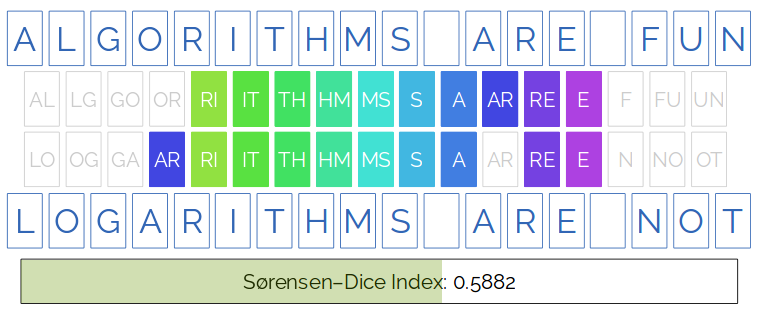
\includegraphics[width=0.75\textwidth]{figuras/dice}
  \caption{Representação da saída do algoritmo de Sørensen–Dice\protect\footnotemark.}
  \label{fig:dice_example}
\end{figure}
\footnotetext{\label{note:dice_example}\textbf{Fonte:} \href{http://www.algomation.com/algorithm/sorensen-dice-string-similarity}{http://www.algomation.com/algorithm/sorensen-dice-string-similarity}.}

O \autoref{dice_index} apresenta uma solução simples e não otimizada para o calculo do coeficiente de Sørensen–Dice na linguagem Python com o uso de {\code sets} para o cálculo do coeficiente em unigramas. Apesar de não ser uma solução ortodoxa do algoritmo e permitir falhas como apontar que as \textit{strings} {\code AA} e {\code AAAA} como idênticas, a solução é interessante para apresentar de forma direta o funcionamento do algoritmo, visto a simplicidade que ele passa a ter quando implementado com {\code sets} e utilizando do operador lógico {\code and} para identificar as interseções entre as \textit{strings}.

\begin{lstlisting}[language=Python,label=dice_index,caption={Simples implementação do coeficiente de Sørensen–Dice}]
def dice_coefficient(a, b):
    """dice coefficient 2nt/na + nb."""
    a_unigram = set(a)
    b_unigram = set(b)
    overlap = len(a_unigram & b_unigram)
    return overlap * 2.0/(len(a_unigram) + len(b_unigram))
\end{lstlisting}

% subsubsection s_rensen_dice_coefficient (end)

\subsubsection*{Smith-Waterman} % (fold)
\label{sec:smith_waterman}


Proposto em 1981 por \textit{Temple F. Smith} e \textit{Michael S. Waterman} \cite{smith1981identification} com o intuito de localizar sequências moleculares semelhantes, este algoritmo de programação dinâmica é hoje amplamente utilizado para a localização de regiões similares entre \textit{strings} e nas sequências de proteínas ou nucleotídeos.

O algoritmo trabalha com o alinhamento de \textit{strings} no intuito de  buscar a maior semelhança entre elas. Considerando este fator, é interessante que as duas \textit{strings} contenham uma quantidade de caracteres igual ou próxima, visto que  a \textit{string} com  maior quantidade de caracteres provavelmente terá suas bordas ignoradas no final. Como resultado, podemos obter melhores resultados com comparações de \textit{strings} que os algoritmos de \textit{Leveinstein} quando tratamos de busca por radicais. Todavia uma comparação usando palavras com uma diferença significativa na quantidade de caracteres poderá resultar em uma perda de desempenho devido ao número de permutações necessárias para localizar o melhor alinhamento.

% Explanação em http://en.wikipedia.org/wiki/Smith%E2%80%93Waterman_algorithm
% TODO: Melhorar essa explanação de bosta
\paragraph*{Algoritmo} % (fold)
\label{sub:algoritmo}

De acordo com o artigo de Smith e Waterman \cite{smith1981identification}, o algoritmo pode ser apresentado da seguinte forma: 
Considerando as \textit{strings} $a$ e $b$ de tamanhos $n,m$ respectivamente e $s(a,b)$ a função de similaridade do universo a ser considerado\footnote{Smith considerava apenas as letras \textit{A,C,U,G} devido ao algoritmo ser voltado para identificação de similidades genéticas, todavia a generalização para as demais letras do alfabeto não invalida o algoritmo.}, é montada uma matriz $H$  para encontrar os dois pares com maior grau de similaridade sendo $W_i$ a nota de lacuna\footnote{Também conhecida como \textit{gap-scoring} ou \textit{gap-penalty}.}.

% \begin{equation*}
% 	H_{k0} = H_{0l} = 0 \text{ para } 0\leq k \leq n \text{ e } 0\leq l \leq m.
% \end{equation*}

Valores preliminares de $H$ tem a interpretação de que $H(i,j)$ tem a máxima similaridade de duas \textit{strings} que possuem final $a_i$ e $b_j$ respectivamente. Os valores de $H(i,j)$ podem ser obtidos através das Equações \ref{smith1} e \ref{smith2}:

\begin{eqnarray*}\label{smith1}
	H(i,0) &=& 0, \, \, \, \, 0 \leq i \leq m \\
	H(0,j) &=& 0, \, \, \, \, 0 \leq j \leq n \\
	H(i,j) &=& \text{max}\lbrace A(i,j), B(i,j), C(i,j), 0\rbrace, \, \, \, \, 1 \leq i \leq n \text{ e } 1 \leq j \leq m
\end{eqnarray*}
onde
\begin{eqnarray*}\label{smith2}
		A(i, j) &=& H(i-1,j-1) + s(a_i,b_j) \\
		B(i, j) &=& \underset{k\geq1}{\text{max}} \left\{H(i-k,j) - W_k\right\}\\ 
		C(i, j) &=& \underset{l\geq1}{\text{max}} \left\{H(i,j-l) - W_l\right\}
\end{eqnarray*}

Montada a matriz $H$, para obter o melhor alinhamento, o algoritmo começa com o maior valor na matriz com índice $(i,j)$, retornando em sentido a célula $(0,0)$, seguindo pelos pontos $(i - 1,j), (i, j - 1)$, ou $(i - 1, j - 1)$.

A fórmula para $H(i,j)$ considera as possibilidades de fim da \textit{string} para qualquer $a_i$ ou $b_j$, tal que:

\begin{enumerate}
	\item Se $a_i$ e $b_j$ forem associados, a similaridade será dada pela Equação \ref{smith3}:
	\begin{equation}\label{smith3}
		H_{i-1,j-1} + s(a_i,b_j)
	\end{equation}
	\item Se $a_i$ está ao fim de uma remoção de largura $k$, a similaridade será dada pela Equação \ref{smith4}:
	\begin{equation}\label{smith4}
		H_{i-k,j} - W_k
	\end{equation}
	\item Se $b_i$ está ao fim de uma remoção de largura $l$, a similaridade será dada pela Equação \ref{smith5}:
	\begin{equation}\label{smith5}
		H_{i,j-l} - W_l
	\end{equation}
	\item Por fim são incluídos sentinelas a fim de evitar o cálculo de similaridades negativas.
\end{enumerate}

% subsection implementa_o_do_algoritmo (end)


% subsection algoritimos_inexatos (end)